\documentclass{siproblemset}

% SI Session Information
\course{MTH 1321}       % the course of your SI
\sessionnum{15}         % (optional) specify the session number
\sessiondate{3/26/20}   % the date of the session

\warmup{Concept Review}
\topic{Mean Value Theorem}
\topic{First Derivative Test}
\cooldown{Extrema from Graphs}

% Worksheet Information
\title{Mean Value Theorem\linebreak and Local Extrema}
\sections{Section 4.3}
\withnamespace

\begin{document}
    \maketitle
    
    \activity{Warmup}{Concept Review}{Answer these questions \textbf{alone} then discuss your answers with a partner. Try not to use your notes.}{15 minutes}
    
    \frq{What is the Mean Value Theorem?}
    \Smallsp
    \frq{What is Rolle's Theorem?}
    \Smallsp
    \mcq{When is a function}{
        \task increasing?
        \tinysp
        \task decreasing?
        \tinysp
    }
    \frq{What does the First Derivative Test tell us?}
    \newpage
  
    \activity{Activity 1}{Mean Value Theorem}{Make a \textbf{group of two or three, all with the same colored worksheets,} to answer your assigned question. Then, try to answer the other questions. Try not to use your notes.}{30 minutes}
    
    \mcq{Find $c$ satisfying the conclusions of the Mean Value Theorem for the given function and interval.}{
        \task $y=\sqrt{x},\hspace{0.5cm}[9,25]$
        \hugesp
        \task $y=x\ln{x},\hspace{0.5cm}[1,2]$
        \Largesp
        \task $y=e^{-2x},\hspace{0.5cm}[0,3]$
        \Hugesp
        \tinysp
        \task $y=x^3,\hspace{0.5cm}[-5,4]$
        \Largesp
    }
\newpage

    \activity{Activity 2}{Local Extrema}{Make a \textbf{group of two or three, all with different colored worksheets,} to answer your assigned question. Then, try to answer the other questions. Try not to use your notes.}{30 minutes}
    
    \mcq{Find all critical points of $f$ and use the First Derivative Test to determine whether they are local minima or local maxima. Also state the intervals on which $f$ is increasing and decreasing.}{
        \task $f(x)=x^3+x^{-3}$
        \hugesp
        \task $f(t)=\dfrac{t^3}{t^2-3}$
        \Largesp
        \tinysp
        \task $f(\theta)=\theta+\sin\theta+\cos\theta$\ \ \ (only consider $0\leq\theta<2\pi$)
        \Hugesp
        \tinysp
        \task $f(x)=\arctan{x}-\frac12x$
    }
\newpage
    
    \activity{Cooldown}{Extrema from Graphs}{Do this problems \textbf{alone}.}{15 minutes}
    \begin{multipartquestion}
        Use the graph below to answer parts (a) through (c).
        
        \begin{center}
            \mbox{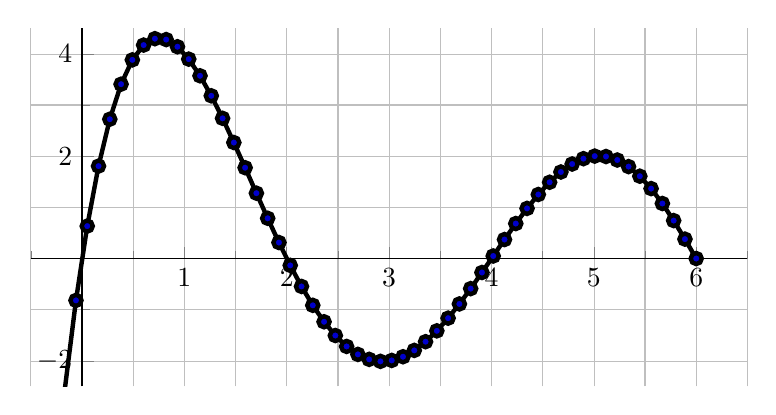
\begin{tikzpicture}[baseline=(current bounding box.north)]
                \begin{axis}[
                x=1.3cm,
                y=0.65cm,
                xmin=-0.5,
                xmax=6.5,
                ymin=-2.5,
                ymax=4.5,
                grid=both,
                major grid style={line width=.2pt,draw=gray!50},
                minor tick num=1,
                axis x line*=middle,
                axis y line*=middle,
                every axis plot/.append style={ultra thick},
                samples=60
                ]
                \addplot+[black, domain=-0.5:6] {13.0667*x-11.9778*x^2+3*x^3-0.0277778*x^4-0.0666667*x^5+0.00555556*x^6};
                \end{axis}
                \end{tikzpicture}}
        \end{center}
        \frq{Determine the intervals on which $f'(x)$ is positive and negative, assuming that the graph above is the graph of $f$. Explain how you got your answer.}
        \Smallsp
        \frq{Determine the intervals on which $f$ is increasing or decreasing, assuming that the graph above is the graph of $f'$. Explain how you got your answer.}
        \Smallsp
        \frq{State whether $f(2)$ and $f(4)$ are local minima or local maxima, assuming that the graph above is the graph of $f'$. Explain how you got your answer.}
    \end{multipartquestion}
    
\end{document}